\documentclass[12pt]{article}
\usepackage{amsmath}
\usepackage{amssymb}
\usepackage{geometry}
\usepackage{amsmath, amsfonts, bm, graphicx}
\usepackage{tabularx}
\usepackage{booktabs} 
\usepackage{float}
\usepackage{enumitem,cancel}
\geometry{margin=1in}

\title{}
\date{}
\author{}

\begin{document}
\subsection*{\boxed{\text{HW 6 - Zeshui Song}}}

\underline{Note:}\\
\textbf{Source Free RC and RL Circuit Response}\\
RC and RL circuits with a single energy storage element (a single capacitor or a single inductor):
\begin{enumerate}
    \item Determine the time constant using a Thevenin equivalent circuit.
    \[\tau_c = R_{\text{Th}} C, \quad \tau_L = \frac{L}{R_{\text{Th}}}\]
    \item Find the initial conditions ($v_0$ for RC circuits and $i_0$ for RL circuits).
    \item Solution:
    \[v(t) = v_0 e^{-\frac{t}{\tau}}, \quad i(t) = i_0 e^{-\frac{t}{\tau}}\]
\end{enumerate}
\textbf{Driven RC Circuit Step Response}
\begin{enumerate}
    \item With all independent sources zeroed out, simplify the circuit to determine $R_{\text{eq}}$ and $C_{\text{eq}}$, and the time constant $\tau_{\text{eq}} = R_{\text{eq}} C_{\text{eq}}$.
    \item Determine the initial condition $v(0^+)$ or $i(0^+)$ [recall that the capacitor voltage is continuous: $v_c(0^-) = v_c(0^+)$]
    \item Determine the steady state condition $v(\infty)$ or $i(\infty)$.
    \item The final response is given by:
  \[\boxed{\begin{aligned}
    v(t) &= v(\infty) + [v(0^+) - v(\infty)] e^{-t/\tau_{\text{eq}}} \\
    i(t) &= i(\infty) + [i(0^+) - i(\infty)] e^{-t/\tau_{\text{eq}}}
    \end{aligned}}\]
\end{enumerate}
\textbf{Driven RL Circuit Step Response}
\begin{enumerate}
    \item With all independent sources zeroed out, simplify the circuit to determine $R_{\text{eq}}$ and $L_{\text{eq}}$, and the time constant $\tau_{\text{eq}} = L_{\text{eq}}/R_{\text{eq}}$.
    \item Determine the initial condition $v(0^+)$ or $i(0^+)$ [recall the requirement that any inductor current $i_L(0^-) = i_L(0^+)$].
    \item Determine the final condition $v(\infty)$ or $i(\infty)$.
    \item The final response is given by
     \[\boxed{\begin{aligned}
    v(t) &= v(\infty) + [v(0^+) - v(\infty)] e^{-t/\tau_{\text{eq}}} \\
    i(t) &= i(\infty) + [i(0^+) - i(\infty)] e^{-t/\tau_{\text{eq}}}
    \end{aligned}}\]
\end{enumerate}


\section*{8.2}
\vspace{-2em}
\begin{center}
    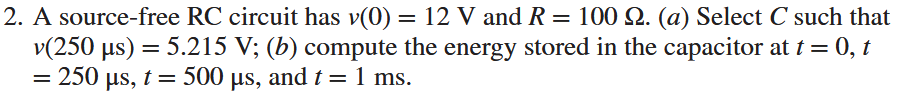
\includegraphics[width=0.8\textwidth]{8-2.png}
\end{center}
\vspace{-1em}
The KCL for a source free RC circuit is given by:
\[C\frac{dv}{dt} + \frac{v}{R} = 0\]
Solving by separating and integrating, we have:
\begin{align*}
    \int \frac{1}{v} dv &= -\int \frac{1}{RC} dt \\
    \ln |v| &= -\frac{t}{RC} + C \\
    v(t) &= e^{C} e^{-\frac{t}{RC}} = C_1 e^{-\frac{t}{RC}}
\end{align*}
Plugging in the initial condition $v(0) = v_0$, we solve for $C_1$:
\[v(0)=C_1 e^{0} = C_1\]
Thus, $C_1 = v_0$, and the solution is:
\[\boxed{v(t) = v_0 e^{-\frac{t}{RC}}}\]
\textbf{(a)} Using the equation for $v(t)$, we plug in the values for $v_0$, $R$, and $v(250\,\mu s)$ to solve for $C$:
\[v(250\times10^{-6}\,\text{s})=[5.215\,\text{V}] = [12\,\text{V}]\exp\left(-\frac{[250\times10^{-6}\,\text{s}]}{[100\,\Omega]C}\right)\]
\[\boxed{C=2.999\times10^{-6}\,\text{F}}\]
\textbf{(b)} The energy stored in the capacitor is given by:
\[w = \frac{1}{2} C v^2\]
\newpage\noindent
The voltages are:
\[v(0)=12\,\text{V}\]
\[v(250\times10^{-6}\,\text{s})=5.215\,\text{V}\]
\[v(500\times10^{-6}\,\text{s})=2.265\,\text{V}\]
\[v(1\times10^{-3}\,\text{s})=0.427\,\text{V}\]
Thus, the energies are:
\[\boxed{\begin{aligned}
    w(0) &= \frac{1}{2} [2.999\times10^{-6}\,\text{F}] [12\,\text{V}]^2 = 2.159\times10^{-4}\,\text{J} \\
    w(250\times10^{-6}\,\text{s}) &= \frac{1}{2} [2.999\times10^{-6}\,\text{F}] [5.215\,\text{V}]^2 = 4.078\times10^{-5}\,\text{J} \\
    w(500\times10^{-6}\,\text{s}) &= \frac{1}{2} [2.999\times10^{-6}\,\text{F}] [2.265\,\text{V}]^2 = 7.692\times10^{-6}\,\text{J} \\
    w(1\times10^{-3}\,\text{s}) &= \frac{1}{2} [2.999\times10^{-6}\,\text{F}] [0.427\,\text{V}]^2 = 2.734\times10^{-7}\,\text{J}
\end{aligned}}\]

\section*{8.8}
\vspace{-2em}
\begin{center}
    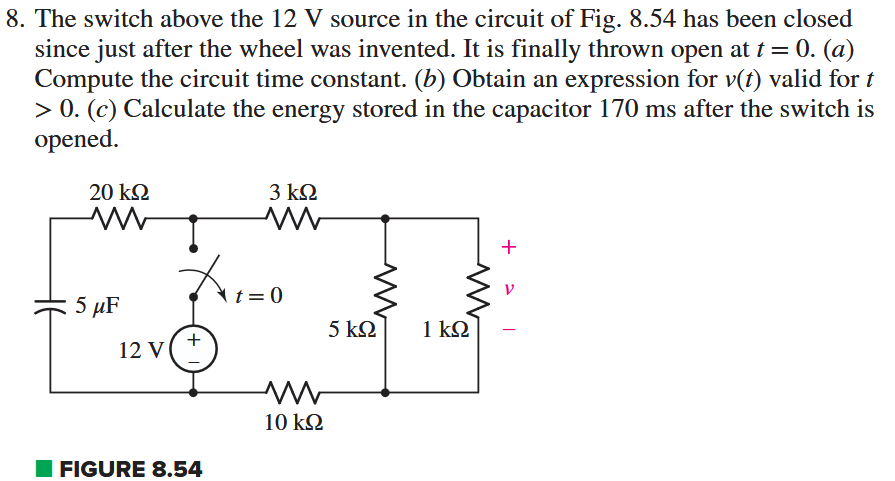
\includegraphics[width=0.8\textwidth]{8-8.png}
\end{center}
\vspace{-1em}
Redrawing the circuit before and after the switch is closed, we have:
\begin{center}
    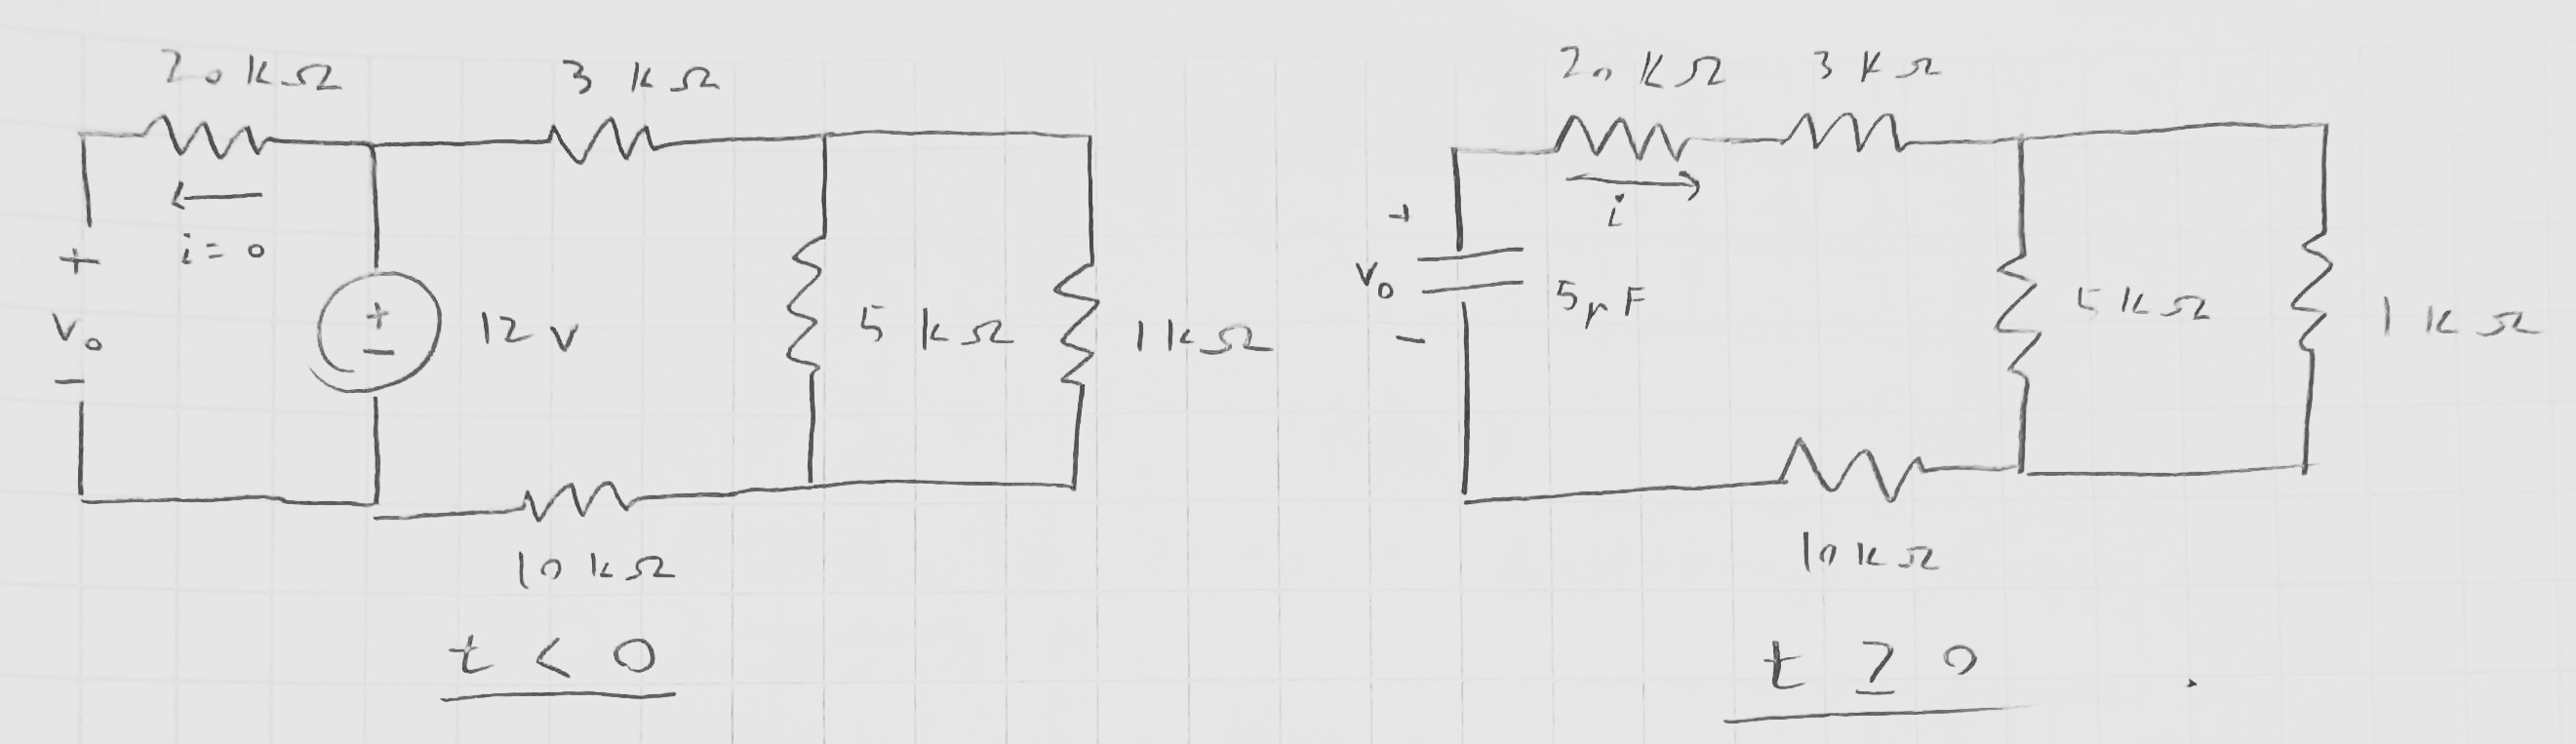
\includegraphics[width=1\textwidth]{8-8-1.jpg}
\end{center}
\underline{Note:} After the switch is flipped, the current will change directions as the capacitor discharges, letting current flow out from its (+) terminal.\\\\
Since a capacitor at steady state behaves like an open circuit, there is no voltage drop across the 20 k$\Omega$ resistor ($i=0$), thus the voltage across the capacitor is $v_0 = 12$ V. \\\\
\textbf{(a)} The time constant is given by: $\tau = R_{\text{Th}} C$. The Thevenin equivalent resistance just the sum of resistances (after opening the switch at t=0) since the source is independent:\\\\
Combine the 1 k$\Omega$ and 5 k$\Omega$ resistors in parallel:
\[R_1 = \frac{[1\cdot5\, k\Omega]}{[1 + 5\, k\Omega]} = 0.833\, k\Omega\]
Combine everything else in series:
\[R_{\text{Th}} = R_1 + [20\, k\Omega]+[3\, k\Omega]+[10\, k\Omega] = 33.833\, k\Omega\]
Thus, the time constant is:
\[\boxed{\tau = R_{\text{Th}} C = [33.833\times10^3\,\Omega] [5\times10^{-6}\,\text{F}] = 169.16\times10^{-3}\, \text{s}}\]
\textbf{(b)} Since we know both $v_0$ and $\tau$, we can solve for the voltage across the capacitor for $t>0$:
\[v_c = 12 \exp\left(-\frac{t}{169.16\times10^{-3}}\right)\]
To find $v(t)$, we can use voltage division for the voltage across the 5 k$\Omega$ - 1 k$\Omega$ parallel combination:
\[v(t) = \frac{R_1}{R_1 + [20\, k\Omega]+[3\, k\Omega]+[10\, k\Omega]} v_c = 0.295\exp\left(-\frac{t}{169.16\times10^{-3}}\right)\]
\[\boxed{v(t) = 0.295\exp\left(-\frac{t}{169.16\times10^{-3}}\right)\,\text{[V]}}\]
\textbf{(c)} The energy stored in the capacitor is given by:
\[w = \frac{1}{2} C v_c^2\]
\[v_c(170\times10^{-3}\,\text{s}) = 12 \exp\left(-\frac{170\times10^{-3}}{169.16\times10^{-3}}\right) = 4.392\,\text{V}\]
\[w(170\times10^{-3}\,\text{s}) = \frac{1}{2} [5\times10^{-6}\,\text{F}] [4.392\,\text{V}]^2 = 4.823\times10^{-5}\,\text{J}\]
\[\boxed{w(170\times10^{-3}\,\text{s}) = 4.823\times10^{-5}\,\text{J}}\]

\section*{8.20}
\vspace{-2em}
\begin{center}
    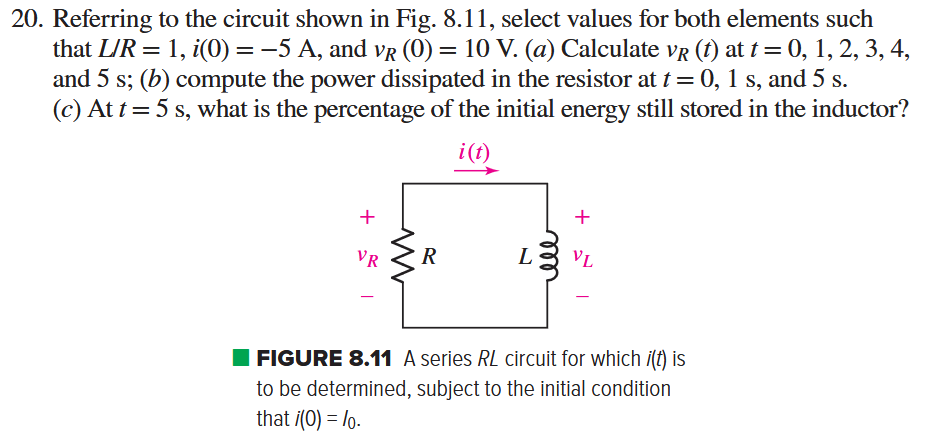
\includegraphics[width=0.8\textwidth]{8-20.png}
\end{center}
\vspace{-1em}
Given:
\begin{itemize}
    \item $\tau=\frac{L}{R}=1$
    \item $i(0)=-5\,\text{A}$
    \item $v_R(0) = 10\,\text{V}$ 
\end{itemize}
The current within the RL circuit is given by:
\[i(t)=i_0\exp\left(-\frac{t}{\tau}\right)=-5\exp(-t)\]
The resistance is then:
\[R=-\frac{v_R(0)}{i(0)} = -\frac{[10\,\text{V}]}{[-5\,\text{A}]} = 2\,\Omega\]
\underline{Note:} Here, the current \textit{doesn't} follow the passive sign convention since it terms the (-) terminal of the resistor instead of the (+) terminal. Thus, Ohms law becomes $v_R = -iR$.
The inductance is then:
\[L=R\quad\implies \quad L=2\,\text{H}\]
\textbf{(a)} The voltage across the resistance is then:
\[v_R(t) = i(t) R = -5\exp(-t) \cdot 2 = -10\exp(-t)\]
\[\boxed{\begin{aligned}
    v_R(0) &= -10\exp(0) = -10\,\text{V} \\
    v_R(1) &= -10\exp(-1) = -3.678\,\text{V} \\
    v_R(2) &= -10\exp(-2) = -1.353\,\text{V} \\
    v_R(3) &= -10\exp(-3) = -0.497\,\text{V}  \\
    v_R(4) &= -10\exp(-4) = -0.183\,\text{V} \\
    v_R(5) &= -10\exp(-5) = -0.067\,\text{V}
\end{aligned}}\]
\textbf{(b)} Power dissipated by the resistor is given by:
\[P_R = \frac{V_R^2}{R}\]
\[\boxed{\begin{aligned}
    P(0) &= \frac{[10\,\text{V}]^2}{2\,\Omega} = 50\,\text{W} \\
    P(1) &= \frac{[3.678\,\text{V}]^2}{2\,\Omega} = 6.763\,\text{W} \\
    P(5) &= \frac{[0.067\,\text{V}]^2}{2\,\Omega} = 0.002\,\text{W}
\end{aligned}}\]
\textbf{(c)} The energy stored in the inductor is given by:
\[w = \frac{1}{2} L i^2\]
Thus,
\[w(0) = \frac{1}{2} [2\,\text{H}] [-5\,\text{A}]^2 = 25\,\text{J}\]
\[w(5) = \frac{1}{2} [2\,\text{H}] [-5\exp(-5)]^2 = 0.00113\,\text{J}\]
Percentage of energy left in the inductor at $t=5$ s is given by:
\[\frac{w(5)}{w(0)} \times 100 = \frac{[0.00113\,\text{J}]}{[25\,\text{J}]} \times 100 = \boxed{0.0045\%}\]

\section*{8.23}
\vspace{-2em}
\begin{center}
    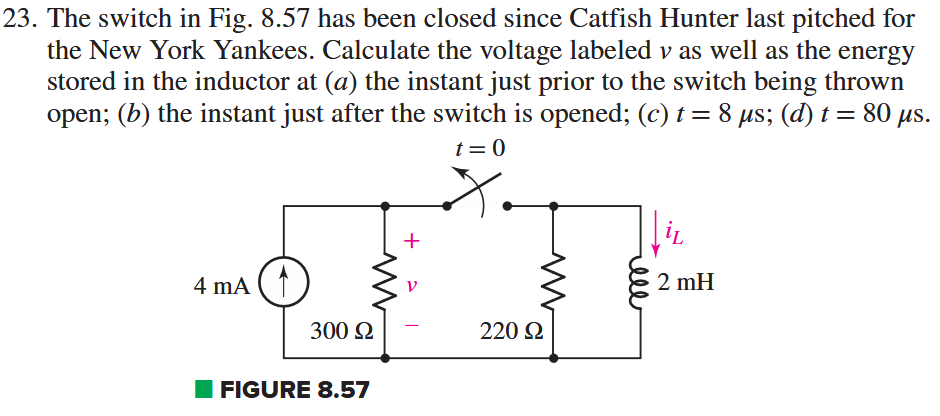
\includegraphics[width=0.8\textwidth]{8-23.png}
\end{center}
\vspace{-1em}
At steady state, the inductor behaves like a short circuit. Since the inductor is in parallel with both the 300 $\Omega$ and 220 $\Omega$ resistors, there will be ZERO current through either resistor because current flows through the path of least resistance. 
\[\implies i_L(0)=4\,\text{mA}\]
\begin{center}
    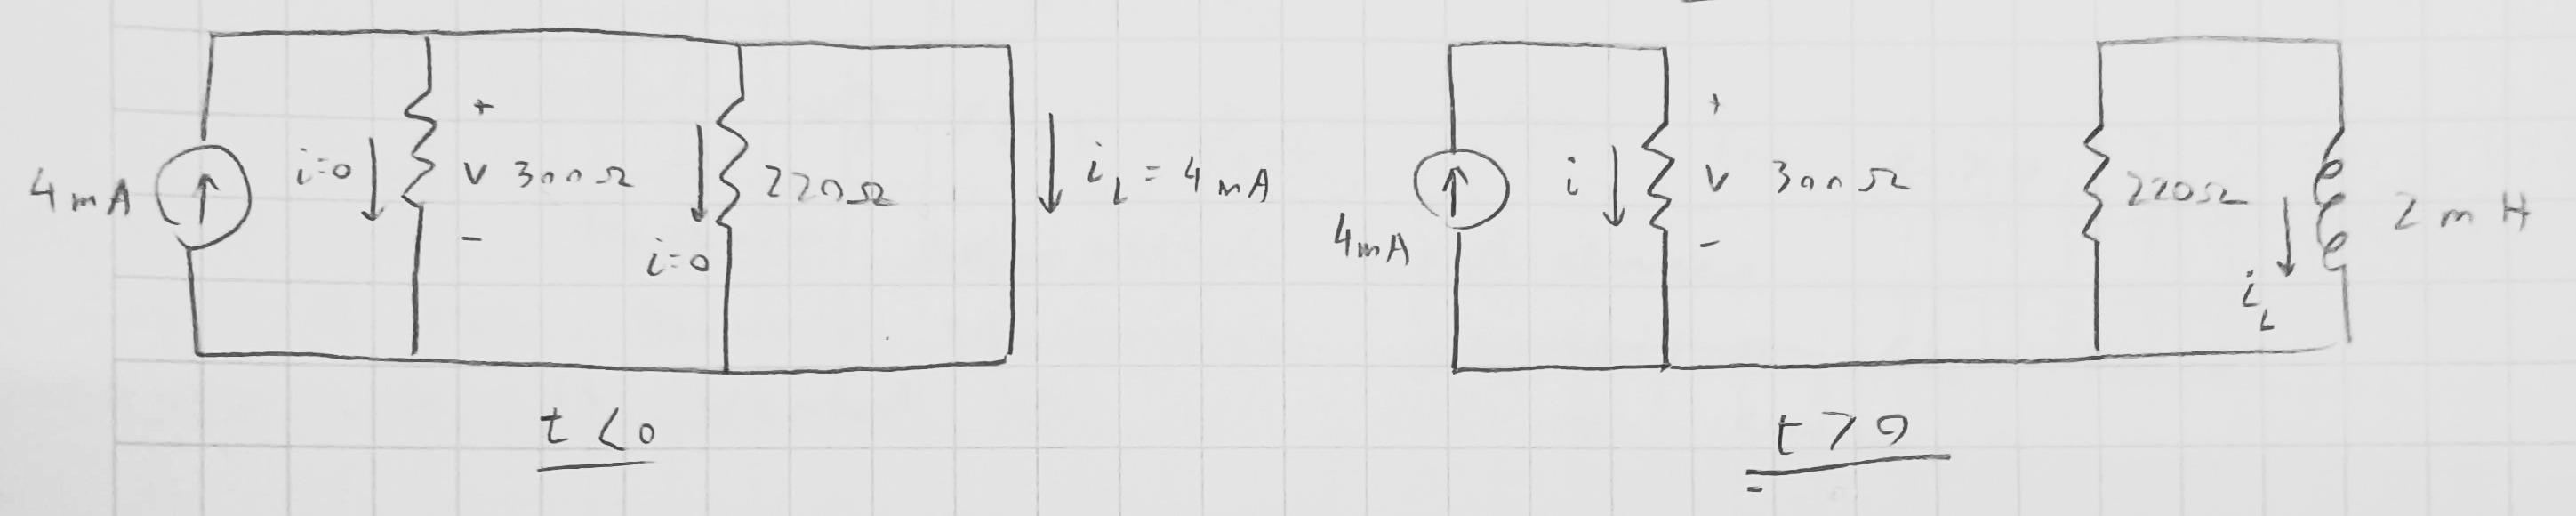
\includegraphics[width=1\textwidth]{8-23-1.jpg}
\end{center}
\underline{Note:} Inductors resist changes in current, so after being disconnected, it will continue to supply current in the same direction as before.\\\\
\textbf{(a)} Just before the switch is open:
\[\boxed{v = 0}\]
The energy stored in the inductor is given by:
\[w = \frac{1}{2} L i_L^2 = \frac{1}{2} [2\times10^{-3}\,\text{H}] [4\times10^{-3}\,\text{A}]^2 = \boxed{16\times10^{-9}\,\text{J}}\]
\textbf{(b)} Just after the switch is open:
\[\boxed{v = iR = [4\times10^{-3}\,\text{A}] \cdot [300\,\Omega] = 1.2\,\text{V}}\]
Time constant is given by:
\[\tau = \frac{L}{R} = \frac{[2\times10^{-3}\,\text{H}]}{[220\,\Omega]} = 9.09\times10^{-6}\,\text{s}\]
Thus,
\[i_L(t) = i_L(0) \exp\left(-\frac{t}{\tau}\right) = (4\times10^{-3}) \exp\left(-\frac{t}{9.09\times10^{-6}}\right)\]
Since the current hasn't changed yet (t=0), the energy stored in the inductor is still:
\[w = \boxed{16\times10^{-9}\,\text{J}}\]
\textbf{(c) \& (d)} Using the formula for current:
\[i_L(8\times10^{-6}) = (4\times10^{-3}) \exp\left(-\frac{8\times10^{-6}}{9.09\times10^{-6}}\right) = 1.658\times10^{-3}\,\text{A}\]
\[i_L(80\times10^{-6}) = (4\times10^{-3}) \exp\left(-\frac{80\times10^{-6}}{9.09\times10^{-6}}\right) = 0.602\times10^{-6}\,\text{A}\]
Thus, the energies are:
\[w(8\times10^{-6}) = \frac{1}{2} L i_L^2 = \frac{1}{2} [2\times10^{-3}\,\text{H}] [1.658\times10^{-3}\,\text{A}]^2 = \boxed{2.748\times10^{-9}\,\text{J}}\]
\[w(80\times10^{-6}) = \frac{1}{2} L i_L^2 = \frac{1}{2} [2\times10^{-3}\,\text{H}] [0.602\times10^{-6}\,\text{A}]^2 = \boxed{3.624\times10^{-16}\,\text{J}}\]
The voltage is constant for the left hand side:
\[\boxed{v = 1.2\,\text{V}}\]

\section*{8.28}
\vspace{-2em}
\begin{center}
    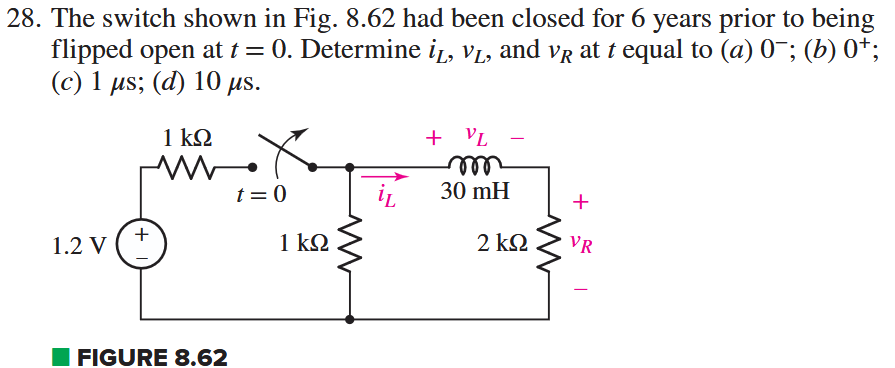
\includegraphics[width=0.8\textwidth]{8-28.png}
\end{center}
\vspace{-1em}
\textbf{(a)} $t=0^-$ (Just before the switch is opened): At steady state, the inductor behaves like a short circuit and $di/dt =0$. Thus,
\[\boxed{V_L = 0}\]
$V_R$ is the same as the voltage across the 1 k$\Omega$-2 k$\Omega$ parallel combination. Thus, by voltage division:
\[R_p = \frac{[1\cdot2\,\text{k}\Omega]}{[1+2\,\text{k}\Omega]} = 0.666\,\text{k}\Omega\]
\[V_R = \frac{[0.666\,\text{k}\Omega]}{[1 + 0.666\,\text{k}\Omega]} \cdot [1.2\,\text{V}] = 0.4801\,\text{V}\]
\[\boxed{V_R = 0.4801\,\text{V}}\]
The current $i_L$ is equal to the current through the 2 k$\Omega$ resistor (series connection):
\[i_L = \frac{V_R}{2\,\text{k}\Omega} = \boxed{0.2401\,\text{mA}}\]
\textbf{(b)} $t=0^+$ (Just after the switch is opened): Not enough time has passed for the current to change, so $i_L$ is still:
\[\boxed{i_L = 0.2401\,\text{mA}}\]
The voltage across the inductor can be found using KVL:
\[-V_L - [2\,\text{k}\Omega] \cdot i_L - [1\,\text{k}\Omega]\cdot i_L = 0 \implies V_L = -0.7202\,\text{V}\]
\[\boxed{V_L = -0.7202\,\text{V}}\]
Also,
\[\boxed{V_R = [2\,\text{k}\Omega] \cdot i_L = 0.4801\,\text{V}}\]
\textbf{(c)} The time constant is given by:
\[\tau = \frac{L}{R} = \frac{[30\times10^{-3}\,\text{H}]}{[3\times10^3\,\Omega]} = 1\times10^{-5}\,\text{s}\]
Thus, the current is given by:
\[i_L(t) = i_L(0) \exp\left(-\frac{t}{\tau}\right) = (0.2401\times10^{-3}) \exp\left(-\frac{t}{1\times10^{-5}}\right)\]
\[\boxed{i_L(10^{-6})=0.2172\times10^{-3}\,\text{A}}\]
Voltage is given by:
\[\implies V_L = L \frac{di_L}{dt} = [30\times10^{-3}\,\text{H}] \cdot \frac{d}{dt} \left[(0.2401\times10^{-3}) \exp\left(-\frac{t}{1\times10^{-5}}\right)\right]\]
\[V_L = -0.7203\exp\left(-\frac{t}{10^{-5}}\right)\]
\[\boxed{V_L(10^{-6}) = -0.6519\,\text{V}}\]
Thus, the voltage across the resistor is:
\[\boxed{V_R(10^{-6}) = [2\,\text{k}\Omega] \cdot i_L(10^{-6}) = 0.4344\,\text{V}}\]
\textbf{(d)} 
\[\boxed{i_L(10\times10^{-6})=0.8832\times10^{-4}\,\text{A}}\]
\[\boxed{V_L(10\times10^{-6}) = -0.2649\,\text{V}}\]
\[\boxed{V_R(10\times10^{-6}) = 0.1766\,\text{V}}\]

\section*{8.35}
\vspace{-2em}
\begin{center}
    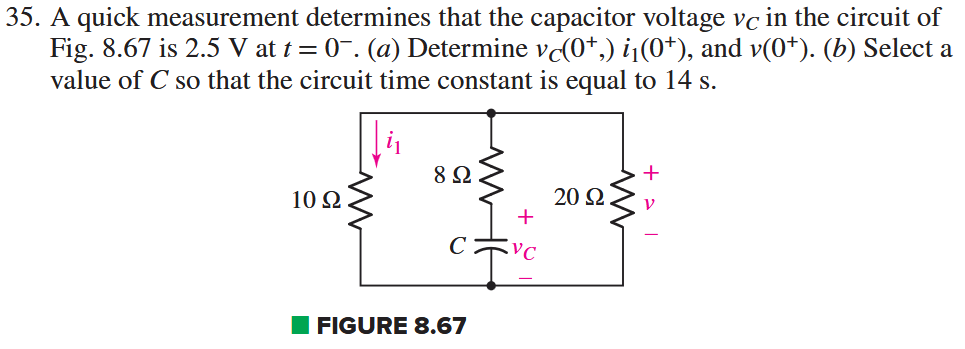
\includegraphics[width=0.8\textwidth]{8-35.png}
\end{center}
\vspace{-1em}
\textbf{(a)} The capacitor voltage is continuous, so
\[\boxed{V_C(0^-) = V_C(0^+)=2.5\,\text{V}}\]
The voltage $V$ is the same as the voltage across the 10 $\Omega$ and 20 $\Omega$ resistors in parallel. Thus, by voltage division:
\[R_p = \frac{[10\cdot20\,\Omega]}{[10+20\,\Omega]} = 6.667\,\Omega\]
\[V(0^+) = \frac{[6.667\,\Omega]}{[6.667+8\,\Omega]} \cdot [2.5\,\text{V}] = \boxed{1.136\,\text{V}}\]
Using Ohm's law:
\[i_1(0^+) = \frac{V_{10\,\Omega}}{[10\,\Omega]} = \frac{1.136\,\text{V}}{10\,\Omega} = \boxed{0.1136\,\text{A}}\]
\textbf{(b)} The time constant is given by:
\[\tau = R_{\text{Th}} C\]
The Thevenin equivalent resistance is the sum of resistances:
\[R_{\text{Th}} = R_p + [8\,\Omega] = 14.667\,\Omega\]
Solving for $C$:
\[C=\frac{\tau}{R_{\text{Th}}}=\frac{[14\,\text{s}]}{[14.667\,\Omega]} = \boxed{0.9545\,\text{F}}\]

\section*{8.46}
\vspace{-2em}
\begin{center}
    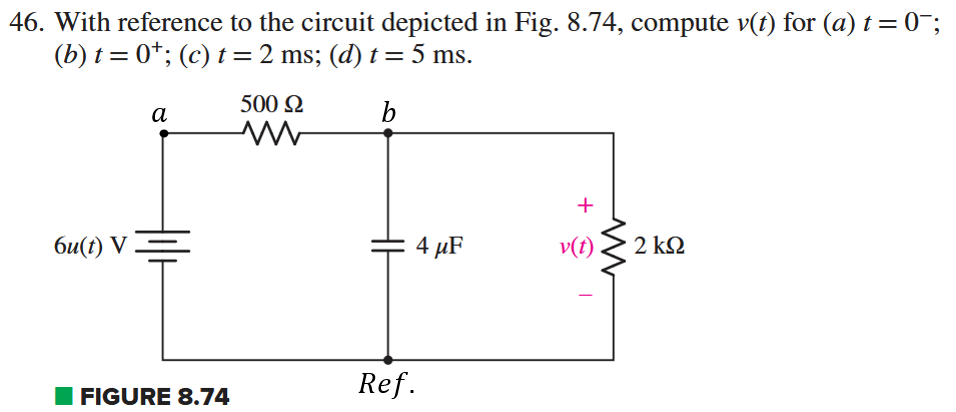
\includegraphics[width=0.8\textwidth]{8-46.png}
\end{center}
\vspace{-1em}
The voltage input is a unit step function, recall that:
\[
u(t - a) =
\begin{cases}
0 & t < a \\
1 & t \ge a
\end{cases}
\]
Thus, at both $t=0^-$ and $t=0^+$, the voltage across the capacitor is zero since it starts uncharged and voltage across a capacitor cannot change instantaneously (it is continuous). Thus, it acts like a short circuit.\\\\
\textbf{(a) \& (b)} Since the capacitor is like a short circuit, for both $t=0^-$ and $t=0^+$, the voltage across the 2 k$\Omega$ resistor in parallel with the resistor is zero.
\[\boxed{V(0^-) = V(0^+) = 0}\]
\textbf{(c)} There are two methods to solve for $v(t)$ for $t>0$:\\\\
\underline{Method 1.} using Nodal analysis (KCL) for $t > 0$ and solving the resulting differential equation:\\\\
Node a:
\[v_a = 6u(t)\,\text{V}\]
Node b:
\[\frac{v_a-v_b}{[500\,\Omega]} = C\frac{dv_c}{dt} + \frac{v_b}{[2\times10^3\,\Omega]}\]
\[\frac{6u(t)-v}{[500\,\Omega]} = [4\times10^{-6}\,\text{F}]\frac{dv_c}{dt} + \frac{v}{[2\times10^3\,\Omega]}\]
Since the capacitor is in parallel with the 2 k$\Omega$ resistor, $v_c = v_b = v$. 
\[\frac{6u(t)-v}{[500\,\Omega]} = [4\times10^{-6}\,\text{F}]\frac{dv}{dt} + \frac{v}{[2\times10^3\,\Omega]} \implies 24u(t) = 0.008\frac{dv}{dt} + 5v\]
Taking the laplace transform:
\[\frac{24u(t)}{s} = 0.008sV(s) + 5V(s) \implies \frac{3000u(t)}{s} = sV(s)+625V(s)\]
\[V(s) = \frac{3000u(t)}{s(s + 625)} = \frac{A}{s} + \frac{B}{s + 625}\quad\text{(Partial fraction)}\]
Solving for $A$ and $B$ using the limit method:
\[A = \lim_{s\to0} s\left(\frac{3000u(t)}{s(s + 625)}\right) = 4.8u(t)\]
\[B = \lim_{s\to-625} (s+625)\left(\frac{3000u(t)}{s(s + 625)}\right) = -4.8u(t)\]
\[V(s) = \frac{4.8u(t)}{s} - \frac{4.8u(t)}{s + 625}\]
Taking the inverse laplace transform:
\[v(t) = 4.8u(t) - 4.8u(t)e^{-625t}\implies \boxed{v(t)=4.8u(t)(1-e^{-625t})\,[\text{V}]}\]
Now we can just plug in the values for $t$ to find the voltage:
\[\boxed{v(2\times10^{-3}) = 3.424\,\text{V}}\]
\textbf{(d)}
\[\boxed{v(5\times10^{-3}) = 4.589 \,\text{V}}\]
\underline{Method 2:} Following the textbook's method for solving driven RC circuits:\\\\
Time constant:
\[\tau = R_{\text{Th}} C\]
The Thevenin equivalent resistance is the sum of resistances:
\[R_{\text{Th}} = \frac{[500\cdot2\times10^3\,\Omega]}{[500 + 2\times10^3\,\Omega]} = 400\,\Omega\]
\[\tau = [400\,\Omega] \cdot [4\times10^{-6}\,\text{F}] = 1.6\times10^{-3}\,\text{s}\]
Initial condition: the capacitor starts uncharged, so
\[v(0^-) = v(0^+) = 0\]
Steady state condition: at $t\to\infty$, the capacitor behaves like an open circuit, so the voltage across the 2 k$\Omega$ resistor is the same as the voltage across the capacitor. By voltage division:
\[v(\infty) = \frac{[2\times10^3\,\Omega]}{[500 + 2\times10^3\,\Omega]} \cdot [6\,\text{V}] = 4.8\,\text{V}\]
By the textbook's formula for driven RC circuits:
\[\boxed{v(t) = v(\infty) + [v(0^+) - v(\infty)] e^{-t/\tau} = 4.8 - 4.8e^{-625t}\,[\text{V}]}\]
This is the same result as Method 1.

\section*{8.50}
\vspace{-2em}
\begin{center}
    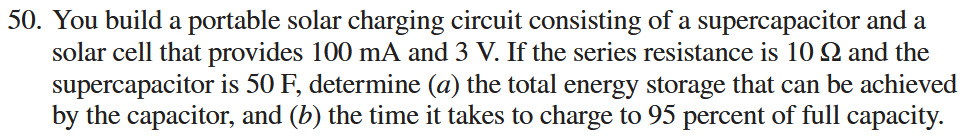
\includegraphics[width=0.8\textwidth]{8-50.png}
\end{center}
\vspace{-1em}
\begin{center}
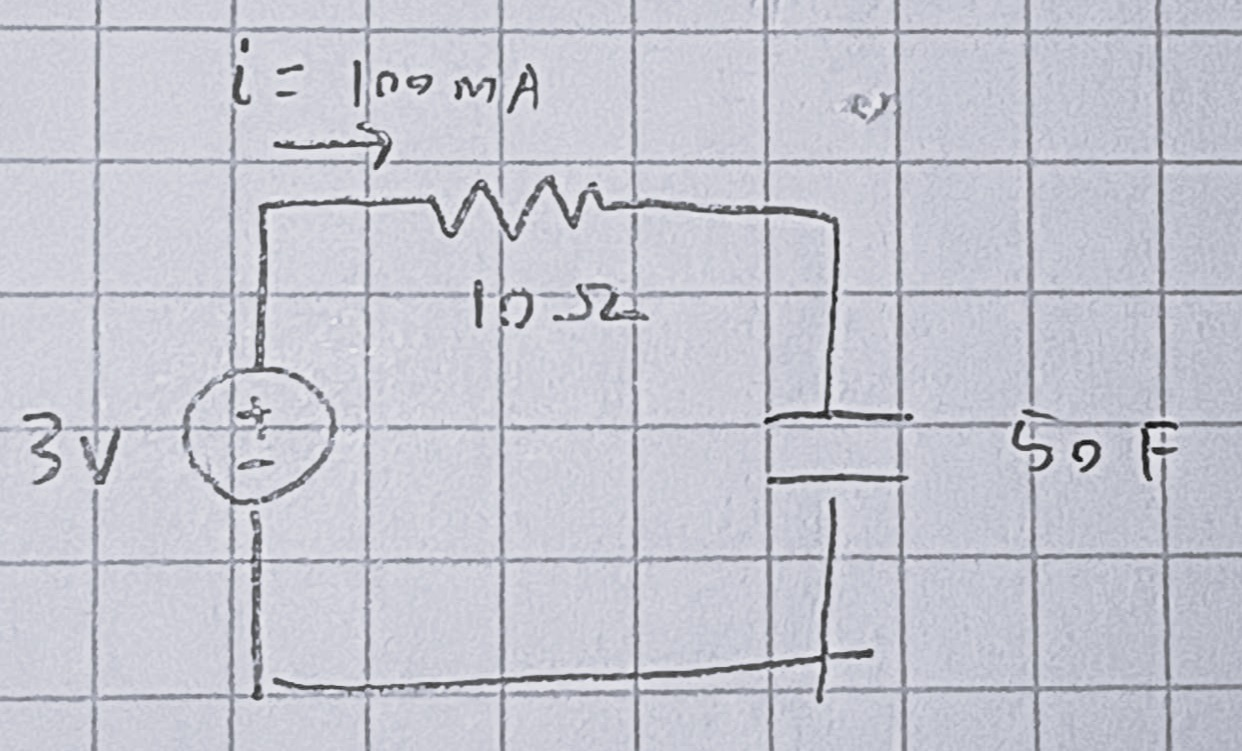
\includegraphics[width=0.5\textwidth]{8-50-1.jpg}
\end{center}
\textbf{(a)} The energy stored in the capacitor is given by:
\[w = \frac{1}{2} C v^2\]
At steady state when the capacitor is fully charged, there is no voltage drop across the 10 $\Omega$ resistor, so the voltage across the capacitor is equal to 3 V.
\[w = \frac{1}{2} [50\,\text{F}] [3\,\text{V}]^2 = \boxed{225\,\text{J}}\]
\textbf{(b)} First we need to find the voltage across the capacitor over time. KCL at the node between the 10 $\Omega$ resistor and the capacitor gives us:
\[\frac{3-v}{[10\,\Omega]}=C\frac{dv}{dt} \implies 0.3 = 0.1v + 50\frac{dv}{dt}\]
Taking the laplace transform:
\[\frac{0.3}{s} = 0.1V(s) + 50sV(s)\]
\[\implies V(s) = \frac{0.3}{s(0.1 + 50s)}=\frac{0.006}{s(0.002+s)}=\frac{A}{s} + \frac{B}{s + 0.002}\quad\text{(Partial fraction)}\]
Solving for $A$ and $B$ using the limit method:
\[A = \lim_{s\to0} s\left(\frac{0.006}{s(0.002+s)}\right) = 3\]
\[B = \lim_{s\to-0.002} (s+0.002)\left(\frac{0.006}{s(0.002+s)}\right) = -3\]
\[V(s) = \frac{3}{s} - \frac{3}{s + 0.002}\]
Taking the inverse laplace transform:
\[\boxed{v(t) = 3 - 3e^{-0.002t}\,[\text{V}]}\]
Plug in $v(t)$ to find time to reach 95\% of the energy stored at steady state:
\[0.95 \cdot 225 = \frac{1}{2} [50\,\text{F}] [v(t)]^2 \implies 8.55 = \left(3 - 3e^{-0.002t}\right)^2\]
\[\implies t = \boxed{1838.06\,\text{s}}\]

\section*{8.54}
\vspace{-2em}
\begin{center}
    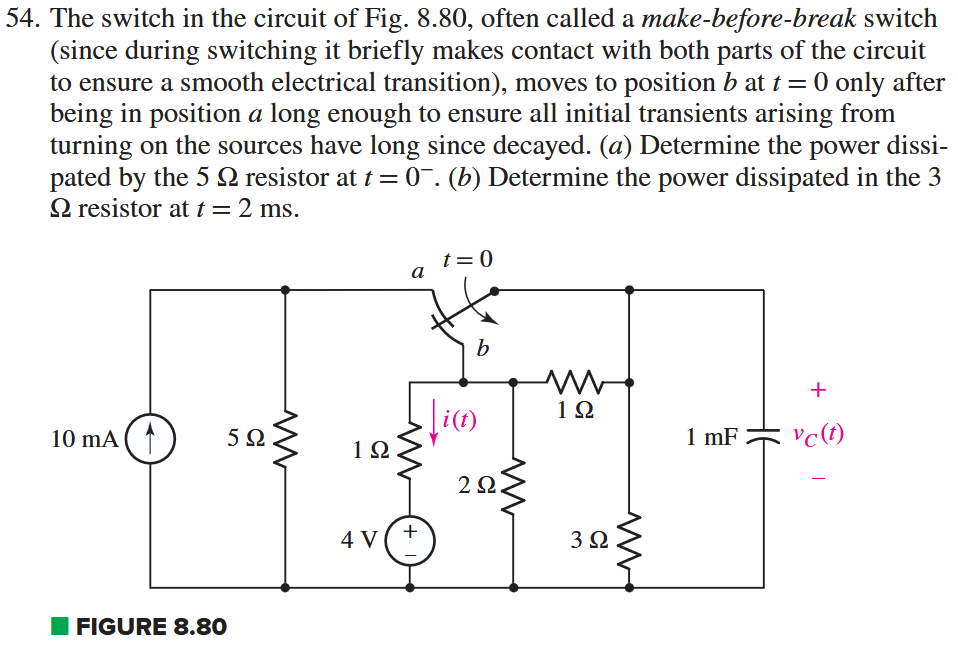
\includegraphics[width=0.8\textwidth]{8-54.png}
\end{center}
\vspace{-1em}
\begin{center}
    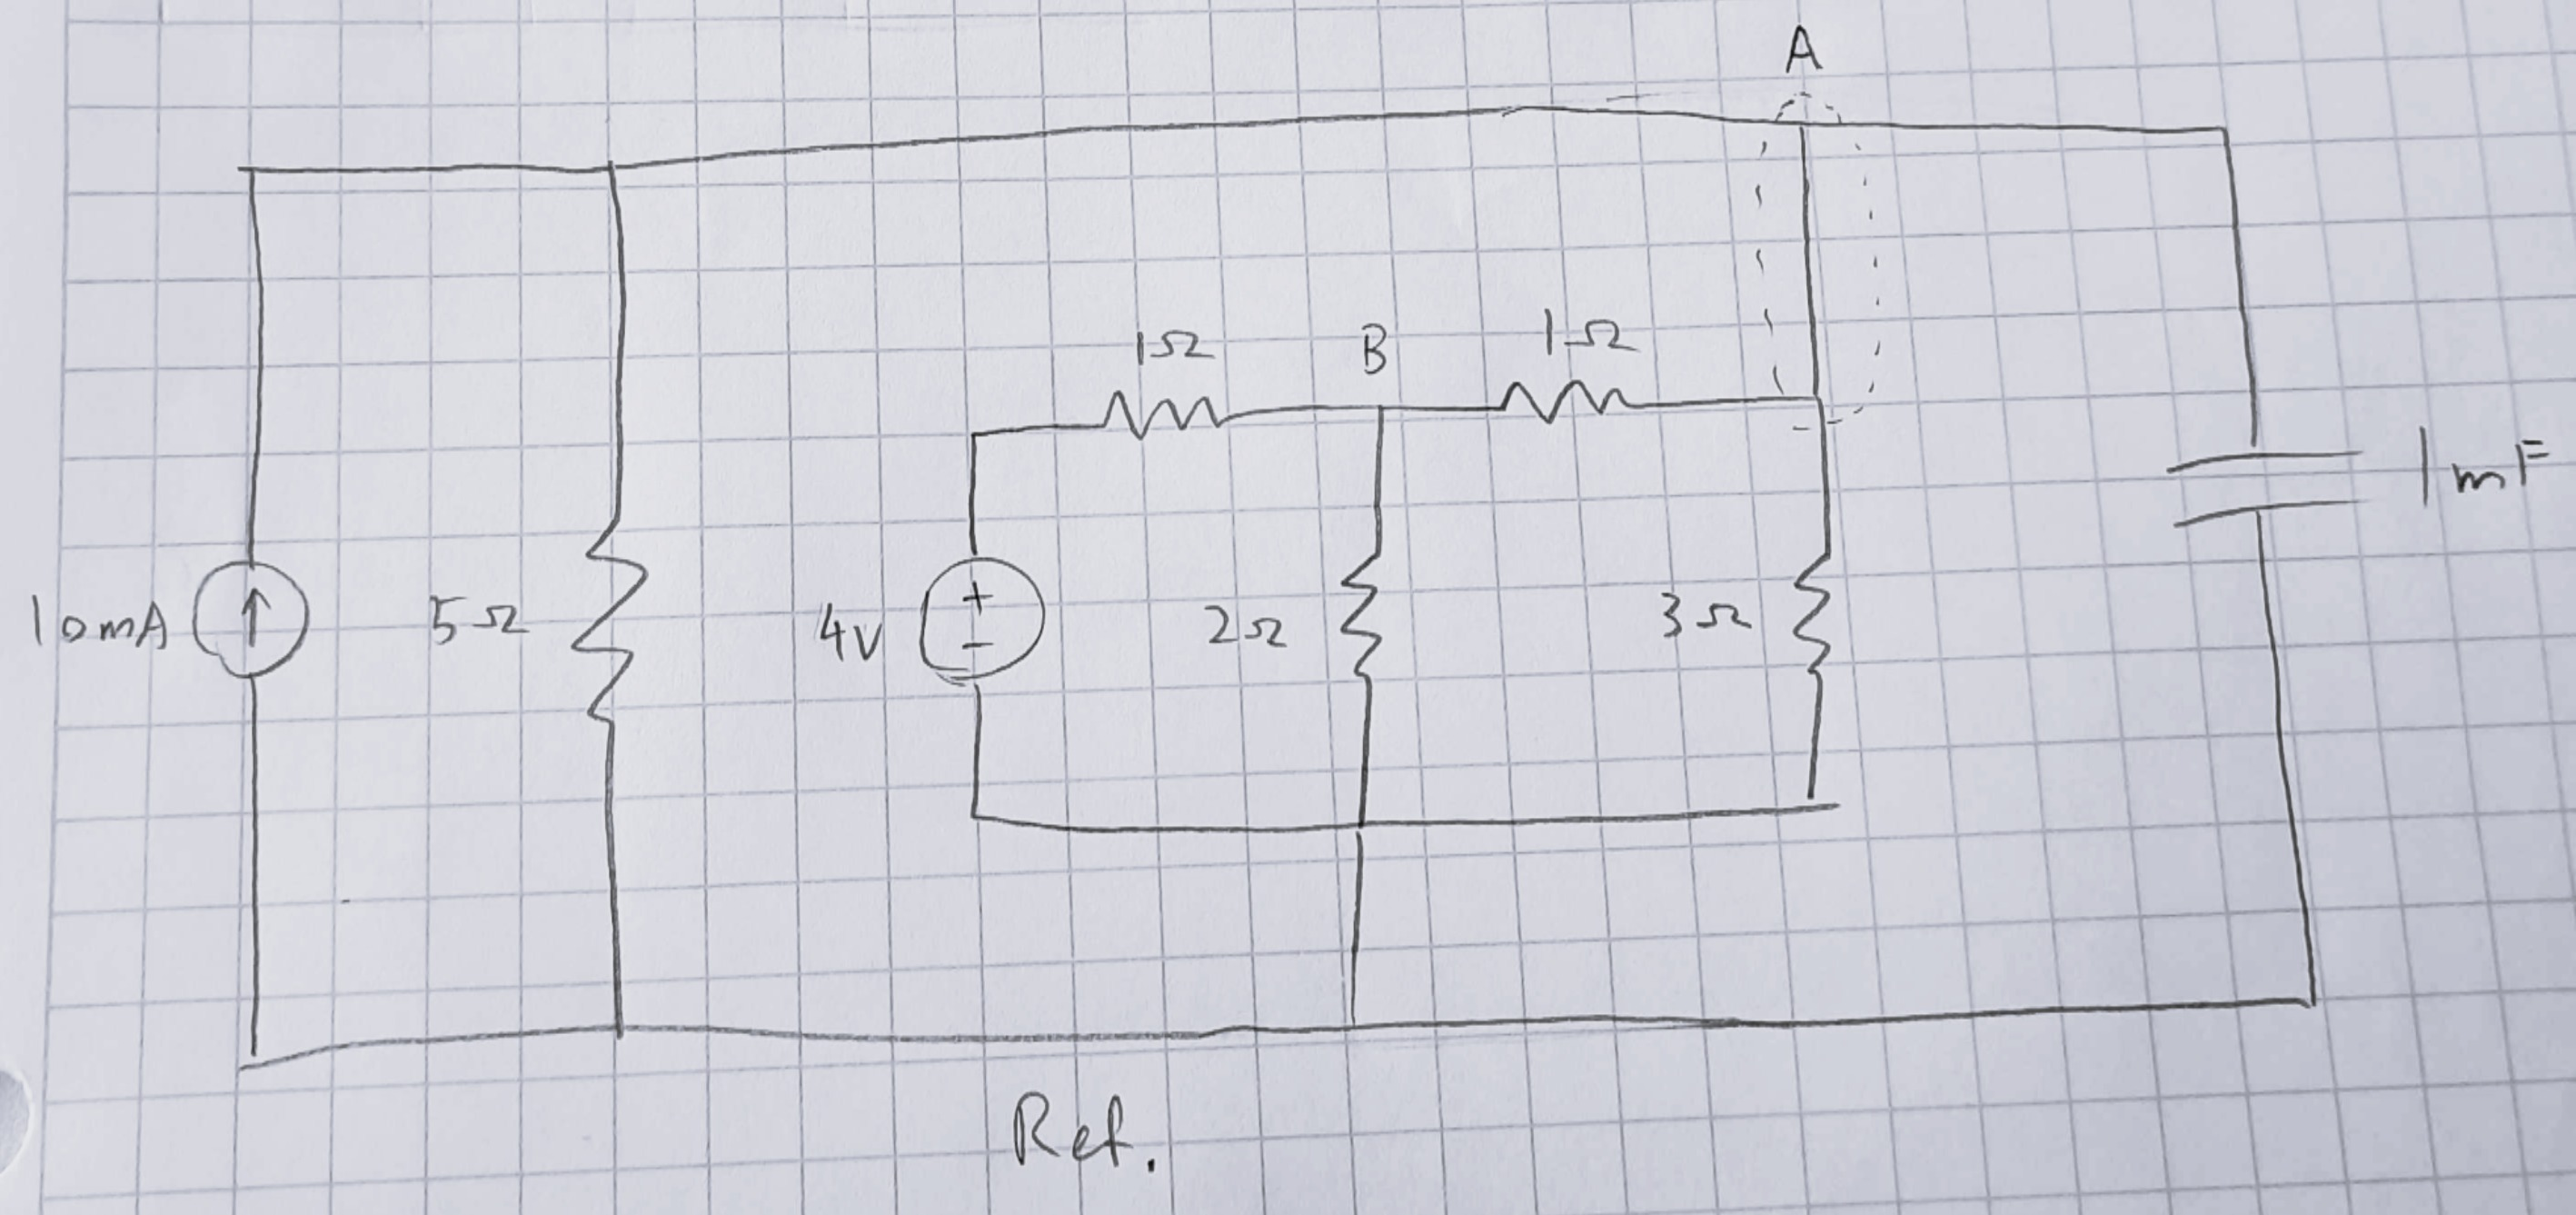
\includegraphics[width=0.8\textwidth]{8-54-1.jpg}
\end{center}
\textbf{(a)} The voltage across the 5 $\Omega$ resistor is equal to $v_A$ so using nodal analysis at steady state:\\\\
Node A:
\[[10\,\text{mA}] = \frac{v_A}{[5\,\Omega]} +\frac{v_A}{[3\,\Omega]}+\frac{v_A-v_B}{[1\,\Omega]}\implies 10\times10^{-3} = \frac{23}{15}v_A-v_B\]
Node B:
\[\frac{v_A-v_B}{[1\,\Omega]}=\frac{v_B-4}{[1\,\Omega]}+\frac{v_B}{[2\,\Omega]}\implies -4=v_A-\frac{5}{2}v_B\]
Solving for $v_A$ and $v_B$:
\[v_A = \boxed{1.4206\,\text{V}}, \quad v_B = \boxed{2.1682\,\text{V}}\]
Thus, the power dissipated by the 5 $\Omega$ resistor is given by:
\[P = \frac{V^2}{R} = \frac{[1.4206\,\text{V}]^2}{[5\,\Omega]} = \boxed{0.4036\,\text{W}}\]
\textbf{(b)} Redrawing the circuit for the switch set to b for $t>0$:
\begin{center}
    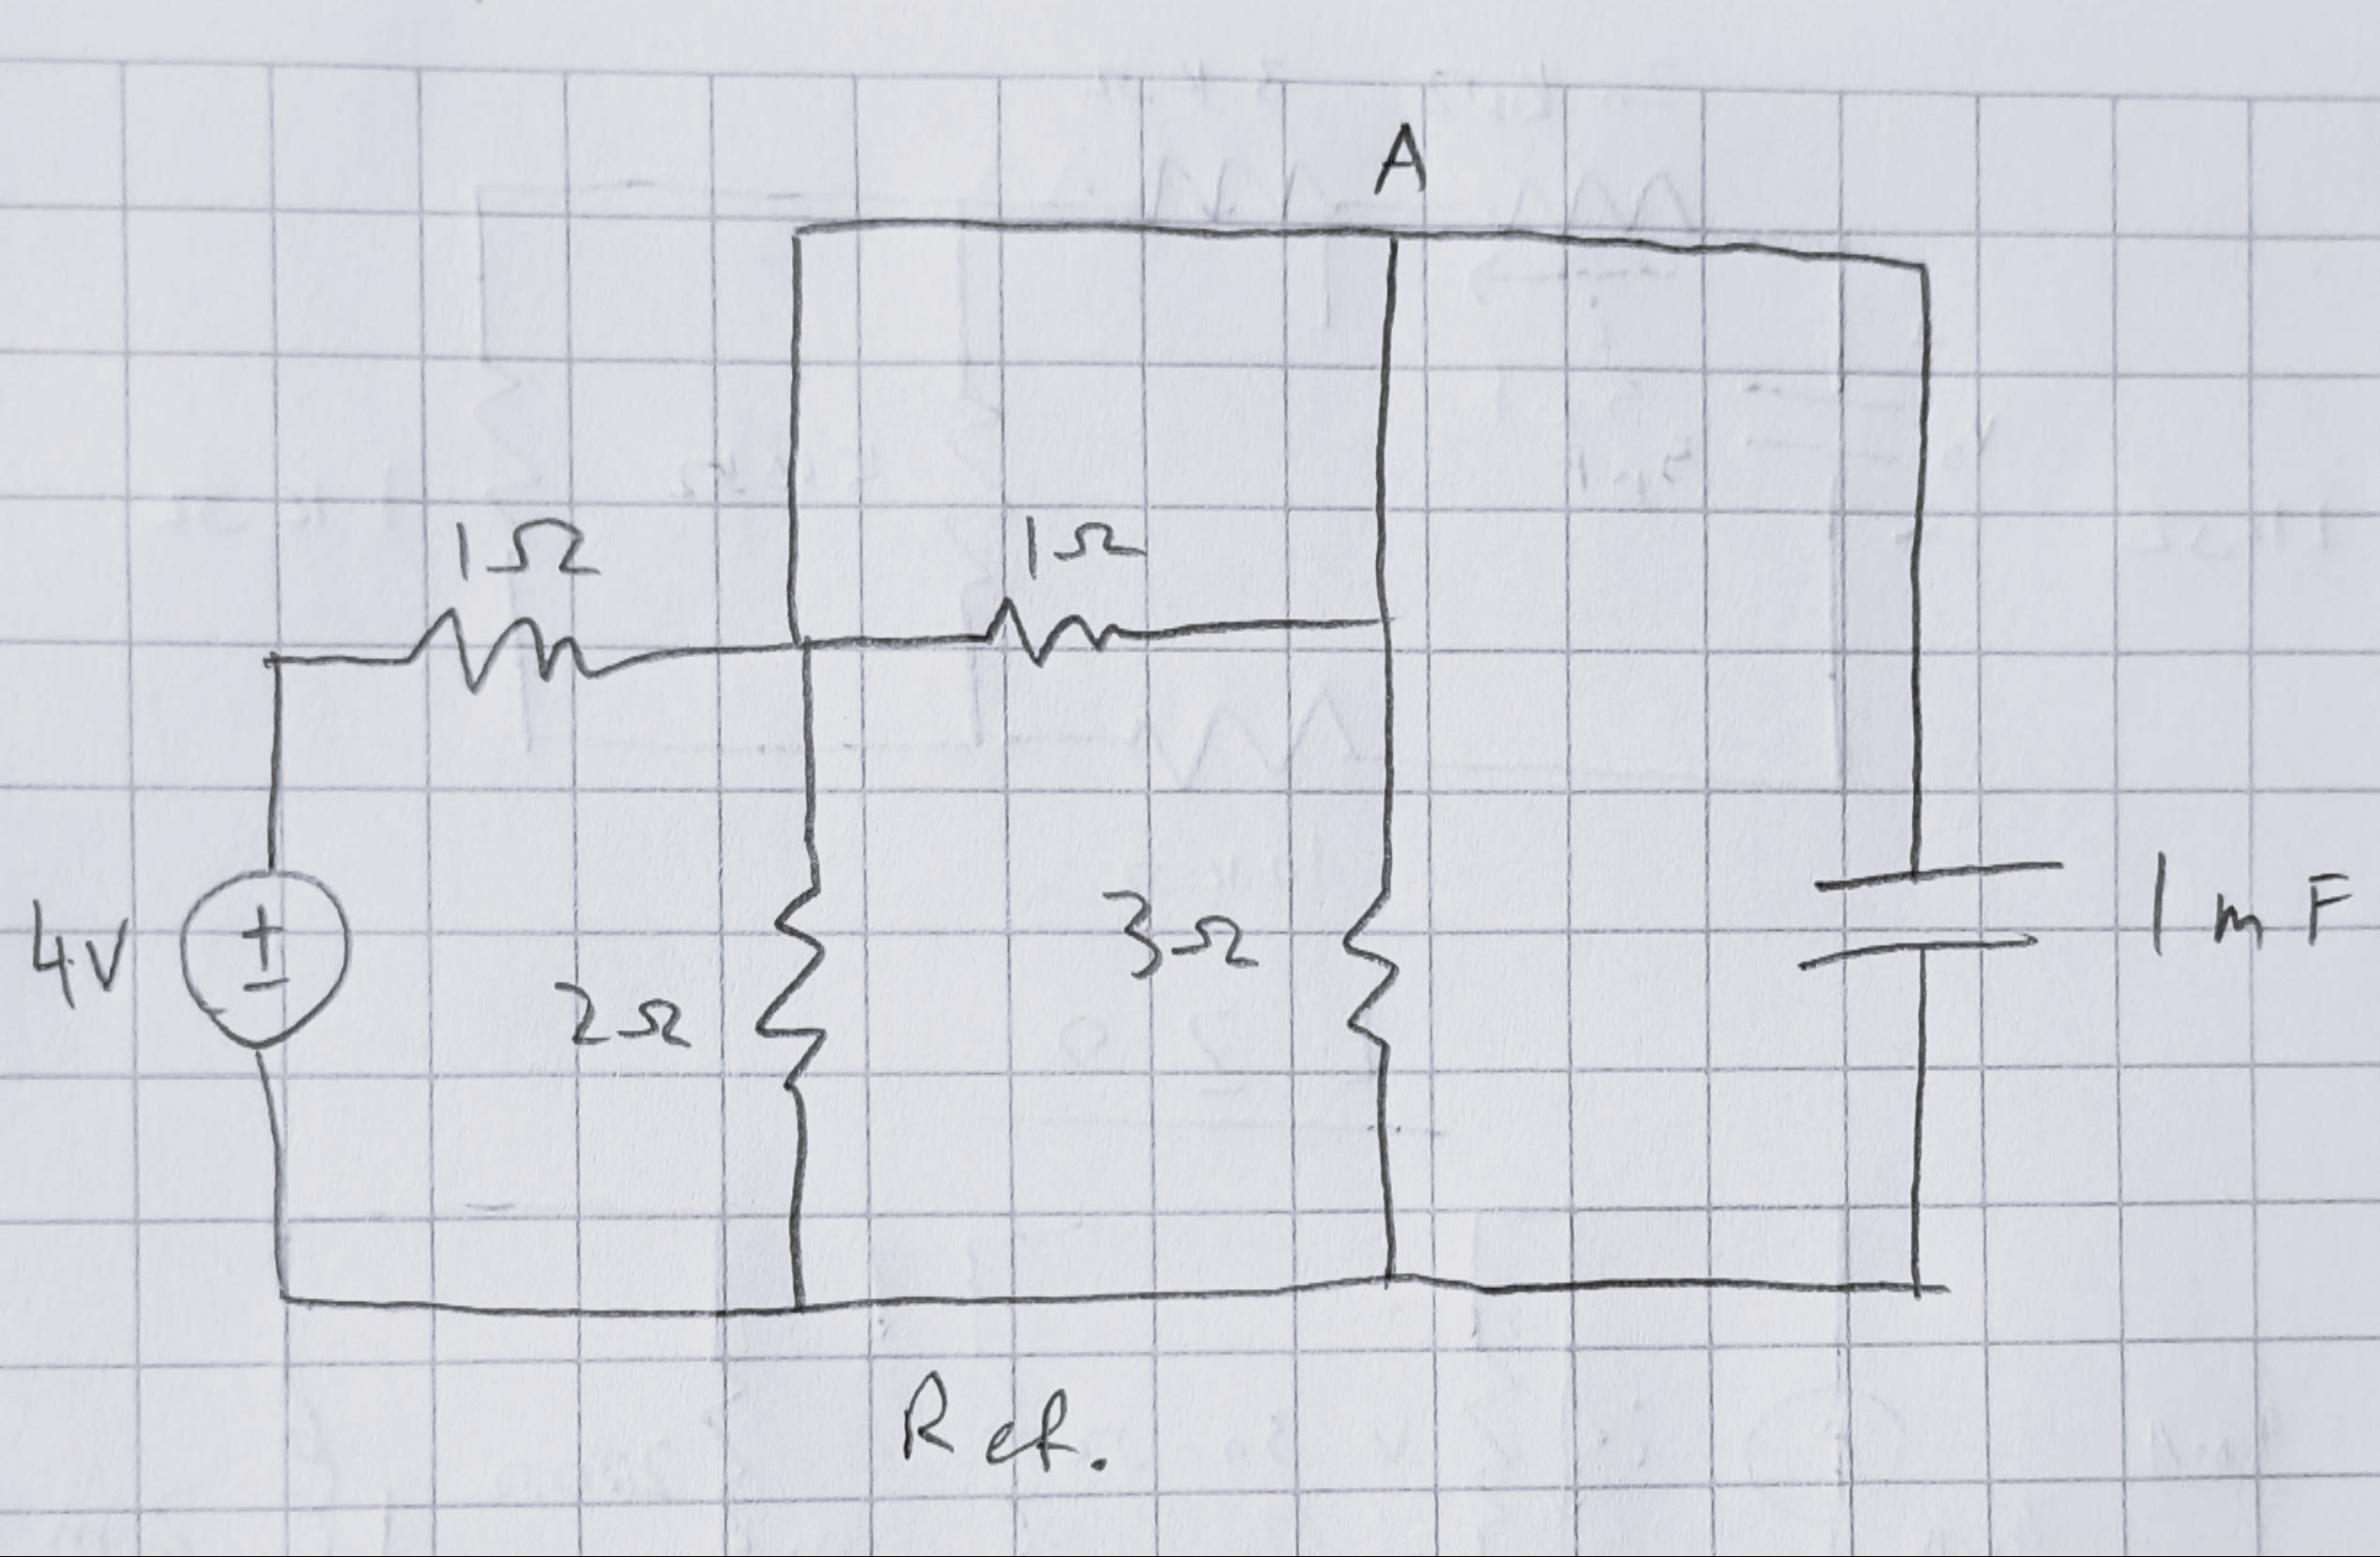
\includegraphics[width=0.5\textwidth]{8-54-2.jpg}
\end{center}
Using KCL at node A:
\[-C\frac{dv_A}{dt} = \frac{v_A}{[3\,\Omega]}+\cancel{\frac{v_A-v_A}{[1\,\Omega]}}+\frac{v_A-4}{[1\,\Omega]}+\frac{v_A}{[2\,\Omega]}\]
\underline{Note:} The capacitor starts off charged and discharges, so the voltage across the capacitor decreases and $dv_A/dt<0$. Thus, I have to put a negative sign to keep the current direction consistent.
\[\implies -10^{-3}\frac{dv_A}{dt} = \frac{11}{6}v_A - 4\]
\[\implies \frac{dv_A}{dt} = -1833.33v_A + 4000\]
Taking the laplace transform:
\[sV_A(s) - v_A(0) = -1833.33V_A(s) + \frac{4000}{s},\quad v_A(0) = 1.4206\,\text{V}\]
\[\implies V_A(s)(s+1833.33)=1.4206 + \frac{4000}{s}\]
\[\implies V_A(s) = \frac{1.4206}{(s+1833.33)} + \frac{4000}{s(s+1833.33)}\]
Partial fraction decomposition for the second term:
\[\frac{4000}{s(s+1833.33)} = \frac{A}{s} + \frac{B}{s+1833.33}\]
Solving for $A$ and $B$ using the limit method:
\[A = \lim_{s\to0} s\left(\frac{4000}{s(s+1833.33)}\right) = 2.18\]
\[B = \lim_{s\to-1833.33} (s+1833.33)\left(\frac{4000}{s(s+1833.33)}\right) = -2.18\]
Thus,
\[V_A(s) = \frac{1.4206}{(s+1833.33)} + \frac{2.18}{s} - \frac{2.18}{s+1833.33} = \frac{-0.7594}{s+1833.33}+\frac{2.18}{s}\]
Taking the inverse laplace transform:
\[\boxed{v_A(t) = 2.18 - 0.7594e^{-1833.33t}\,[\text{V}]}\]
The voltage across the 3 $\Omega$ resistor is the same as $v_A$, so the power dissipated by the 3 $\Omega$ resistor is given by:
\[v_A(2\times10^{-2}) = 2.1605\,\text{V}\]
\[P = \frac{V^2}{R} = \frac{[2.1605\,\text{V}]^2}{[3\,\Omega]} = \boxed{1.556\,\text{W}}\]
\underline{Note:} When applying KCL, I usually use the (Current into node) = (Current out of node) convention. However, for inductors and capacitors, it is hard to figure out the direction. Thus, applying \textit{passive sign convention}, we say that ALL currents are exiting the node and NO current is entering the node. This way, the math will naturally work out, and we don't have to worry about the direction of current for inductors and capacitors (one of the terms will be forced negative).

\section*{8.61}
\vspace{-2em}
\begin{center}
    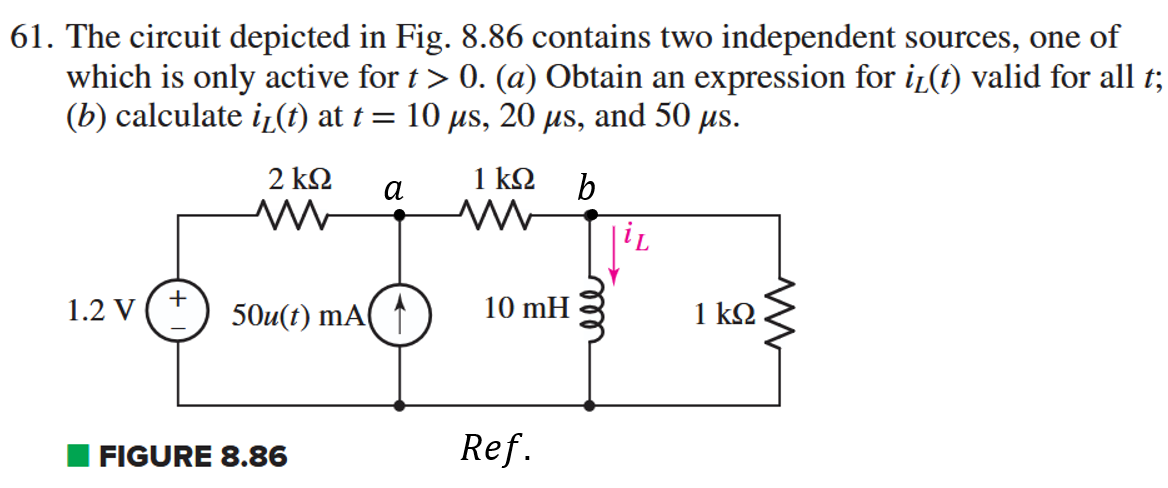
\includegraphics[width=0.8\textwidth]{8-61.png}
\end{center}
\vspace{-1em}
\textbf{(a)} I will try the textbook method for solving driven circuits here. First turning off all the independent sources (voltage sources become short circuits and current sources become open circuits):
\begin{center}
    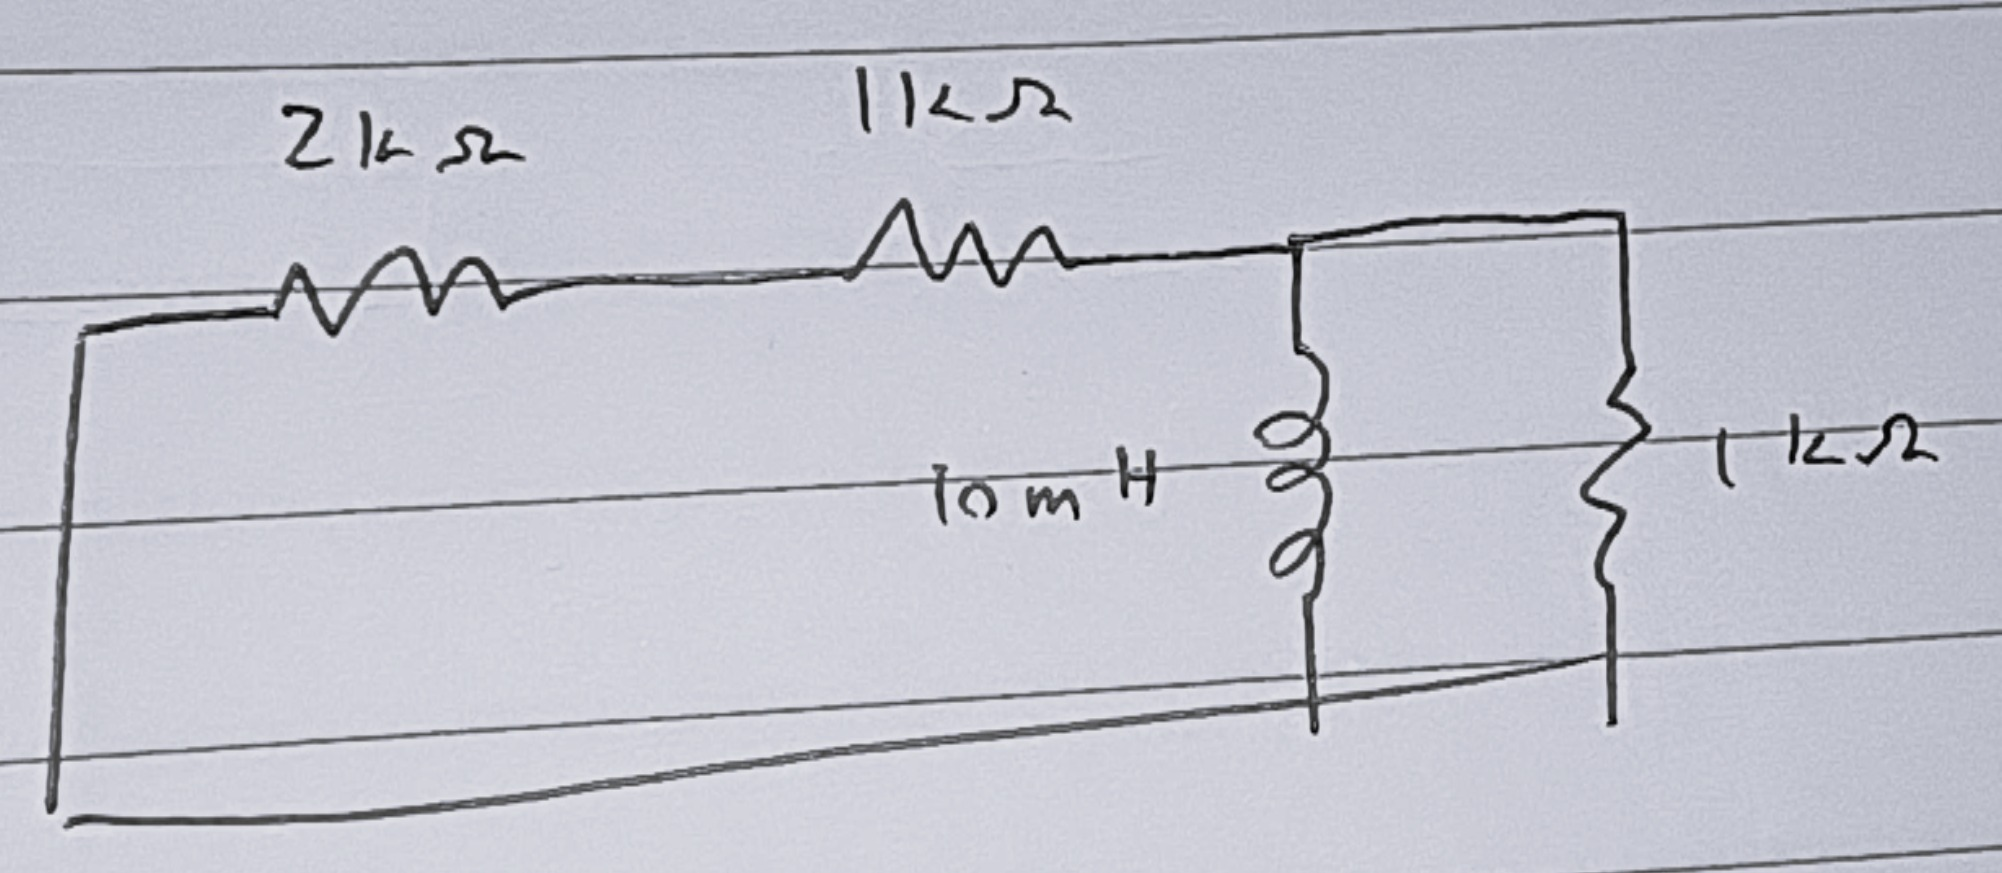
\includegraphics[width=0.5\textwidth]{8-61-1.jpg}
\end{center}
Add 2 k$\Omega$ and 1 k$\Omega$ in series:
\[R = 2+1 = 3\,\text{k}\Omega\]
Add the 3 k$\Omega$ and 1 k$\Omega$ in parallel:
\[R_{\text{eq}}=\frac{3\cdot1}{3+1} = 0.75\,\text{k}\Omega\]
Thus the time constant is given by:
\[\tau = \frac{L_\text{eq}}{R_\text{eq}} = \frac{[10\times10^{-3}\,\text{H}]}{[0.75\times10^3\,\Omega]} = 13.33\times10^{-6}\,\text{s}\]
Now find the initial condition and steady state conditions for the current through the inductor after turning the sources back on.\\\\
Initially ($t = 0$), the inductor behaves like a short circuit under the 1.2 V source, but the second source is still off. Thus, the current through the inductor is the same as the current through both resistors in series:
\[V_s=iR_{\text{eq}} \implies i=i_L(0) = \frac{1.2}{3\times10^3} = 0.4\,\text{mA}\]
At steady state ($t \to \infty$), the inductor behaves like a short circuit, thus the current through the inductor is equal to the current through the 1 k$\Omega$ resistor. Quick mesh analysis gives us:
\begin{center}
    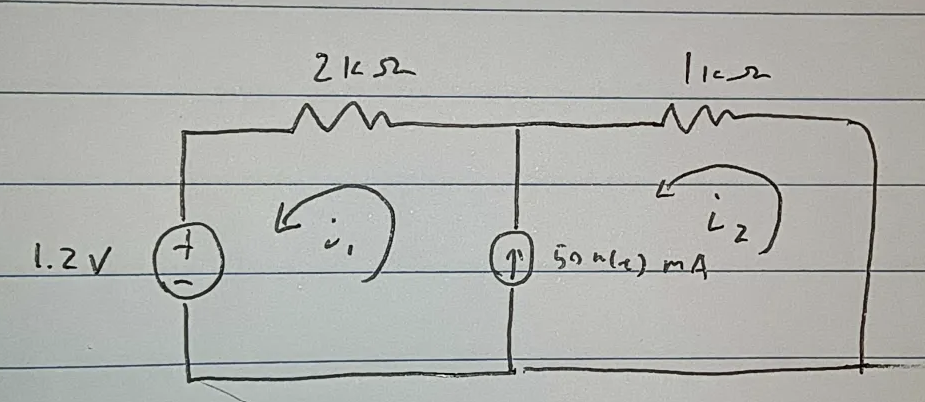
\includegraphics[width=0.6\textwidth]{8-61-2.png}
\end{center}
Supermesh eqn:
\[i_1-i_2 = 50\times10^{-3}\]
\[-[1\,\text{k}\Omega]i_2-[2\,\text{k}\Omega]i_1-[1.2\,\text{V}]=0\]
Solving for $i_1$ and $i_2$:
\[i_1 = 0.01626\,\text{A}, \quad i_2 = -0.0337\,\text{A}\]
Thus, following the sign convention for $i_L$:
\[i_L(\infty) = -i_2 = 0.0337\,\text{A}\]
Finally, using the textbook's formula for driven RL circuits:
\[\boxed{i_L(t) = i_L(\infty) + [i_L(0) - i_L(\infty)] e^{-t/\tau} = 0.0337 - 0.0333e^{-t/(13.33\times10^{-6})}\,[\text{A}]}\]
\textbf{(b)}
\[\boxed{\begin{aligned}
i_L(10\times10^{-6}) &= 17.99\times10^{-3}\,\text{A}\\
i_L(10\times20^{-6}) &= 26.30\times10^{-3}\,\text{A}\\
i_L(10\times50^{-6}) &= 32.95\times10^{-3}\,\text{A}
\end{aligned}}\]

\section*{8.67}
\vspace{-2em}
\begin{center}
    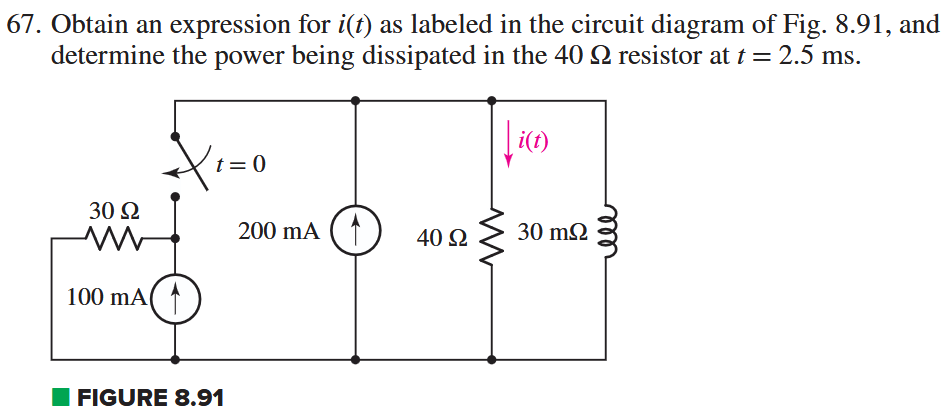
\includegraphics[width=0.8\textwidth]{8-67.png}
\end{center}
\vspace{-1em}
Following the textbook method again, but first find the initial condition (recall that while current is continuous, voltage across an inductor can change instantaneously). Thus the initial voltage is equal to the voltage across the resistors in parallel:
\[R_{\text{eq}} = \frac{30\cdot40}{30+40} = 17.14\,\Omega\]
At $t=0$, $i_L(0^-)=i_L(0^+)=200\,\text{mA}$, so the voltage across the resistors is given by the remaining current:
\[i_\text{source} = i_\text{resistors} + i_L(0^+) \implies i_\text{resistors} = 100\,\text{mA}\] 
\[v_L(0^+) = [17.14\,\Omega] \cdot [100\times10^{-3}\,\text{A}] = 1.714\,\text{V}\]
After $t=0$, the switch is flipped and the time constant is given by:
\[\tau = \frac{L_{\text{eq}}}{R_{\text{eq}}}\]
Turning off the sources to find the equivalent inductance and resistance:
\[R_{\text{eq}} =  17.14\,\Omega\]
\[L_{\text{eq}} = 30\times10^{-3}\,\text{H}\]
\[\tau = \frac{30\times10^{-3}\,\text{H}}{17.14\,\Omega} = 1.75\times10^{-3}\,\text{s}\]
At steady state ($t\to\infty$), the inductor shorts the entire circuit:
\[v_L(\infty) = 0\,\text{V}\]
Thus,
\[\boxed{v_L(t) = v_L(\infty) + [v_L(0) - v_L(\infty)] e^{-t/\tau} = 1.714e^{-t/(1.75\times10^{-3})}\,[\text{V}]}\]
Now, the voltage across the 40 $\Omega$ resistor is the same as the voltage across the inductor, so the power dissipated by the 40 $\Omega$ resistor is given by:
\[v_L(2.5\times10^{-3}) = 0.4107\,\text{V}\]
\[P = \frac{V^2}{R} = \frac{[0.4107\,\text{V}]^2}{[40\,\Omega]} = \boxed{0.004218\,\text{W}}\]

\section*{8.70}
\vspace{-2em}
\begin{center}
    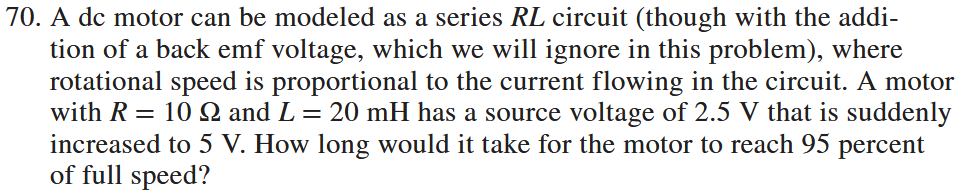
\includegraphics[width=0.8\textwidth]{8-70.png}
\end{center}
\vspace{-1em}
\begin{center}
    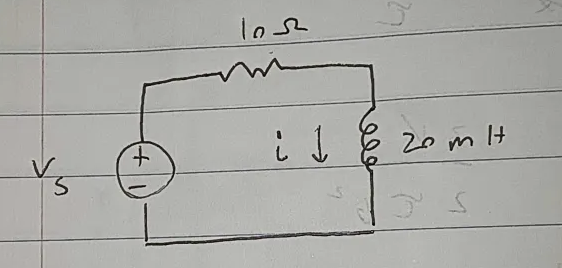
\includegraphics[width=0.5\textwidth]{8-70-1.png}
\end{center}
Given:
\begin{itemize}
    \item $\omega=ki$
    \item $v_s = 2.5+2.5u(t)\,\text{V}$
\end{itemize}
The question asks for \textit{when} the motor reaches 0.95 of full speed. Since motor speed is proportional to the current through the circuit, we simply have to find the time to reach 0.95 of the steady state current.\\\\
Textbook method for solving driven RL circuits again. The time constant is given by:
\[\tau = \frac{L}{R} = \frac{[0.02\,\text{H}]}{[10\,\Omega]} = 0.002\,\text{s}\]
The initial condition is given by the current through the inductor at $t=0^+$ since the current is continuous:
\[i_L(0^-) = \frac{[2.5\,\text{V}]}{[10\,\Omega]} = 0.25\,\text{A}\]
\[i_L(0^+) = i_L(0^-) = 0.25\,\text{A}\]
At steady state ($t\to\infty$):
\[i_L(\infty) = \frac{[2.5+2.5\,\text{V}]}{[10\,\Omega]} = 0.5\,\text{A}\]
Thus, using the textbook's formula for driven RL circuits:
\[\boxed{i_L(t) = i_L(\infty) + [i_L(0) - i_L(\infty)] e^{-t/\tau} = 0.5 - 0.25e^{-t/0.002}\,[\text{A}]}\]
Thus, 0.95 of the steady state current is given by:
\[0.95\cdot0.5 = 0.475\,\text{A}\]
Solve for $t$:
\[0.475 = 0.5 - 0.25e^{-t/0.002} \implies t = \boxed{4.605\times10^{-3}\,\text{s}}\]

\end{document}